\documentclass{article}

\usepackage{geometry}
\usepackage{makecell}
\usepackage{array}
\usepackage{multicol}
\usepackage{setspace}
\usepackage{changepage}
\usepackage{cprotect}
\usepackage{booktabs}
\usepackage{graphicx}
\usepackage{float}
\newcolumntype{?}{!{\vrule width 1pt}}
\newcommand{\paragraphlb}[1]{\paragraph{#1}\mbox{}\\}
\renewcommand\theadalign{tl}
\setstretch{1.10}
\setlength{\parindent}{0pt}


\geometry{top=12mm, left=1cm, right=2cm}
\title{\vspace{-1cm}Netzwerktechnologien Übung 4}
\author{Andreas Hofer}

\begin{document}
	\maketitle
	\section{IP-Adresse}
	\begin{figure}[H]
		\centering
		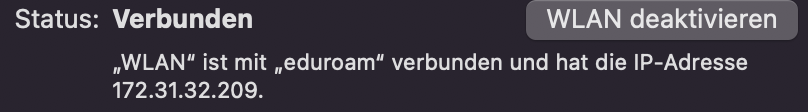
\includegraphics[scale=0.75]{Bilder/ip_address.png}
		\caption{Die IP-Adresse im Uni Netzwerk}
	\end{figure}
	Die IP-Adresse des PCs im Netzwerk ist 172.31.32.209.
	\section{ARP}
	\subsection{Ausgabe des ARP Caches}
	\begin{figure}[H]
		\centering
		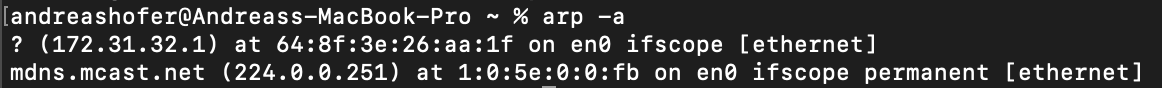
\includegraphics[scale=0.75]{Bilder/arp_cache.png}
		\cprotect\caption{Die Ausgabe des \verb|arp -a|  Befehls.}
	\end{figure}
	\addtocounter{subsection}{2}
	\subsection{ARP Request/Reply}
	\begin{figure}[H]
		\centering
		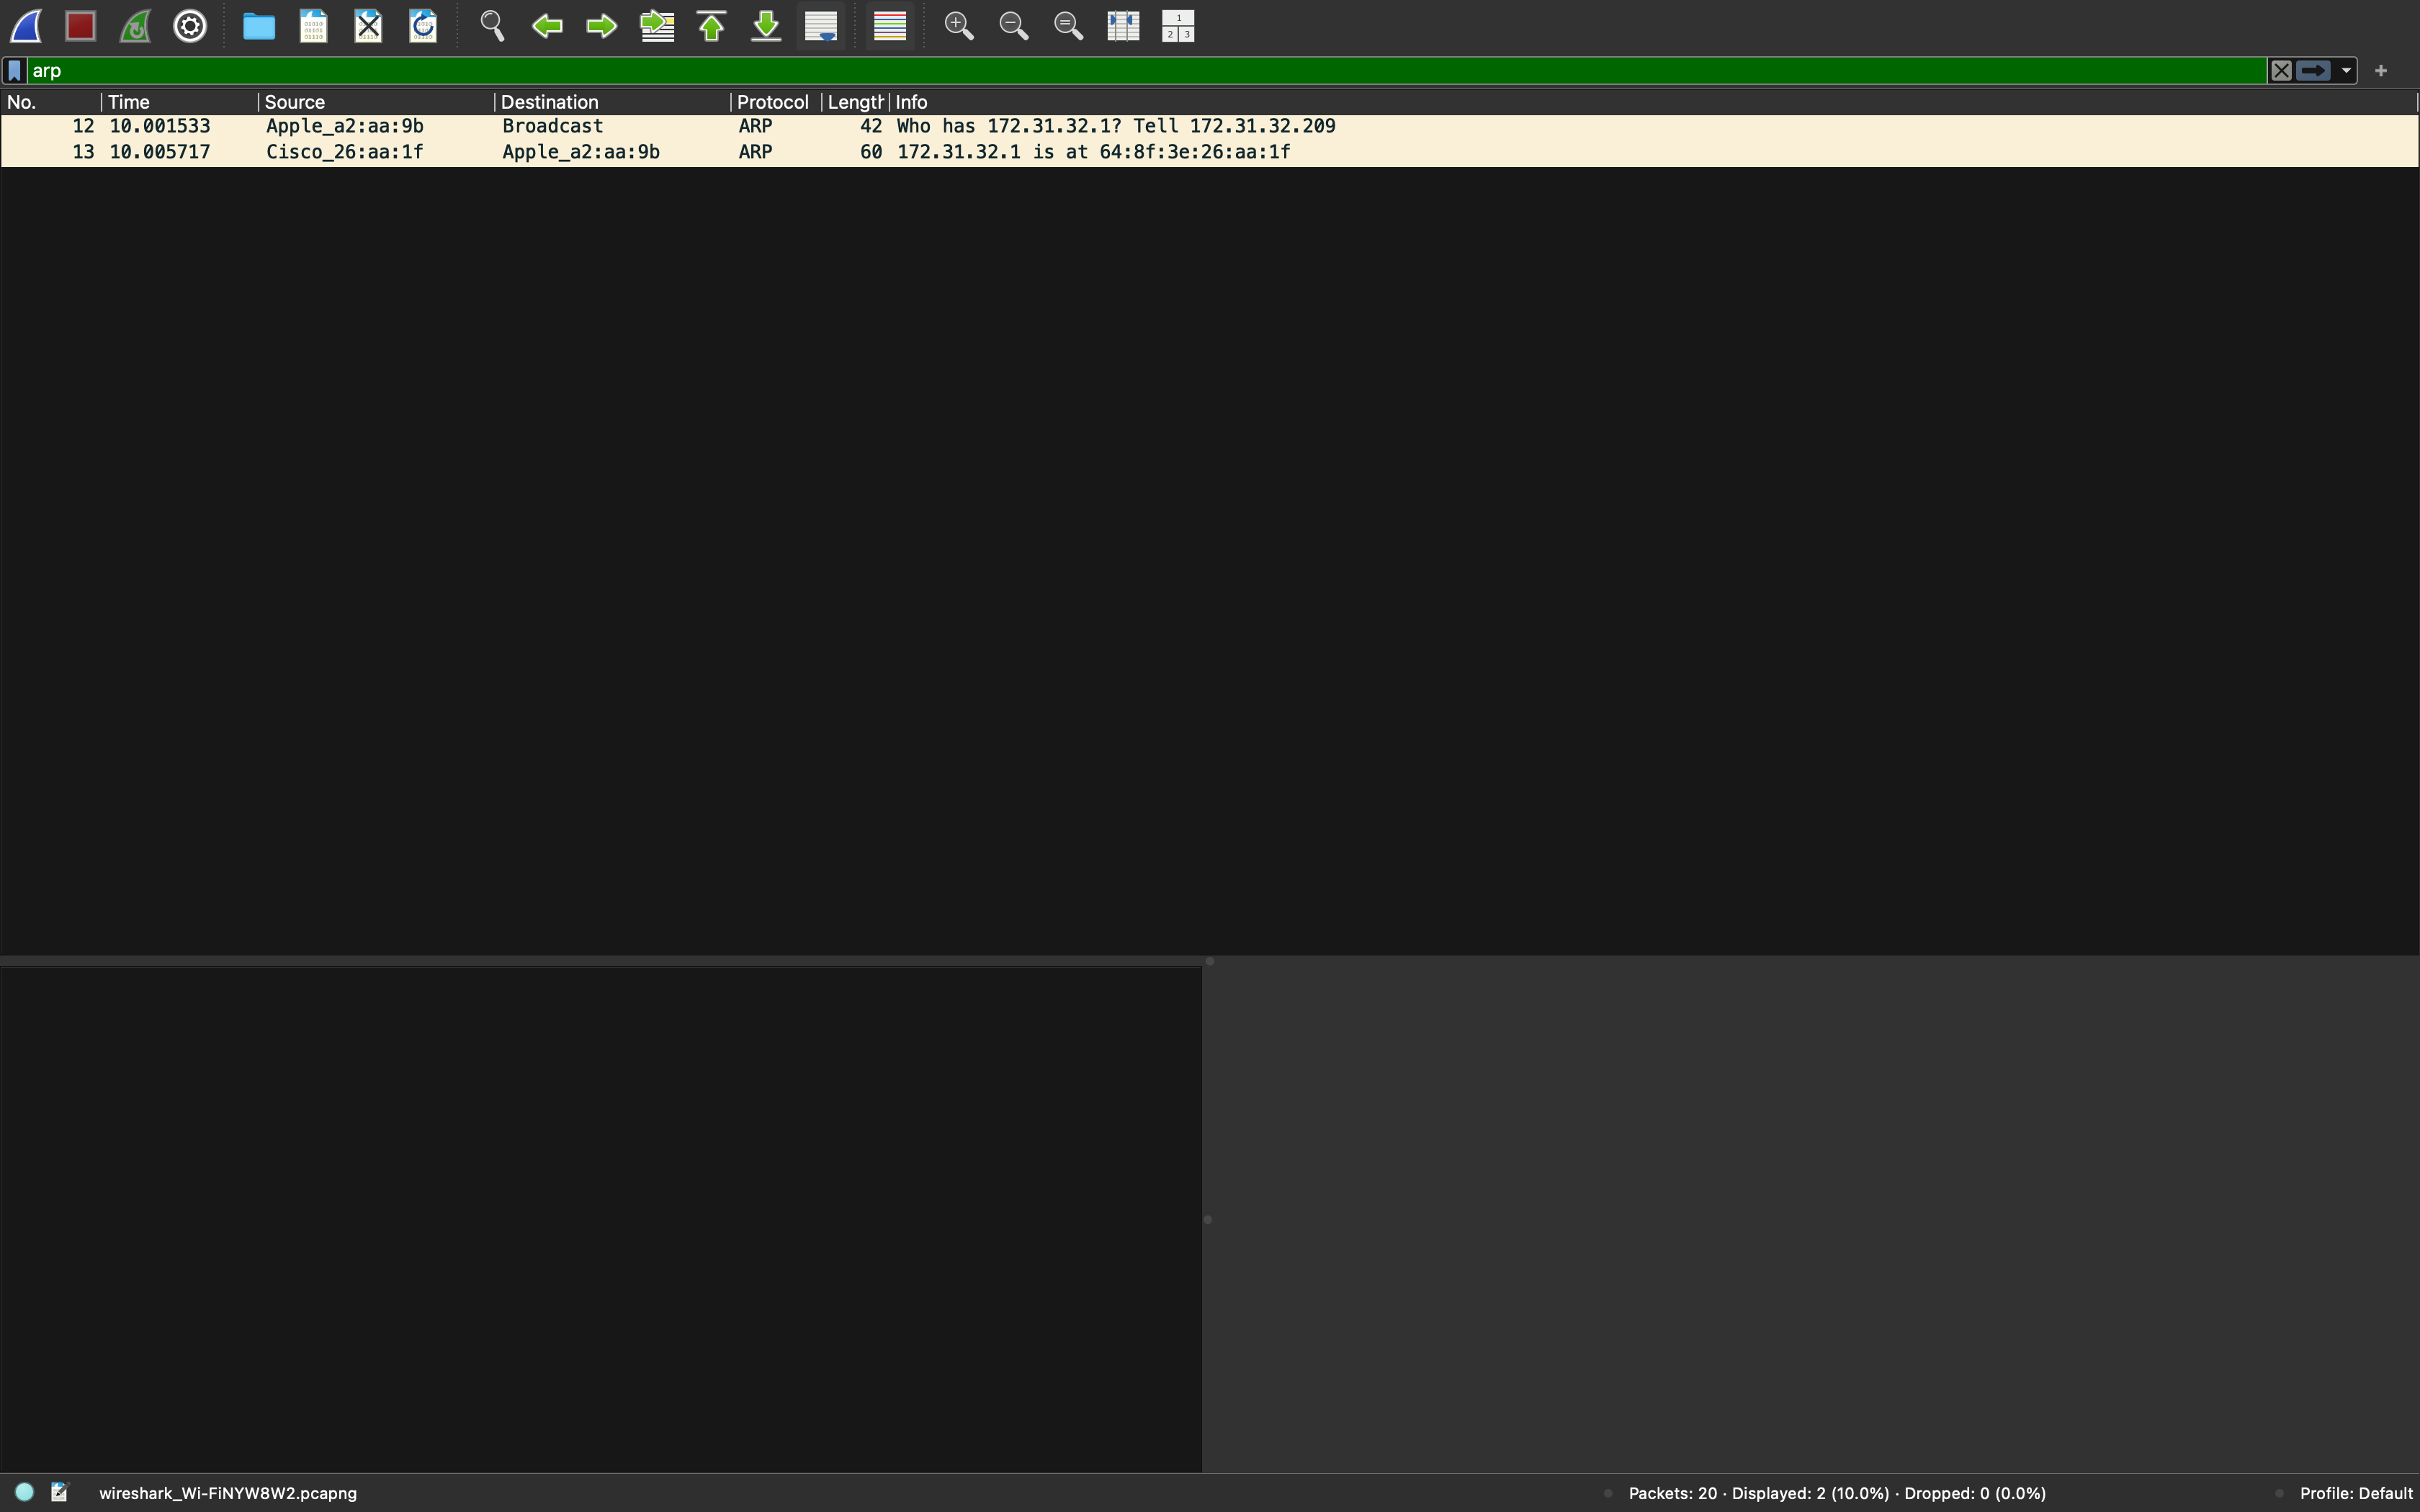
\includegraphics[scale=0.3]{Bilder/arp_request.png}
		\caption{ARP Request und Reply in Wireshark}
	\end{figure}
	\subsection{Request/Reply Paket}
	\begin{figure}[H]
	\centering
	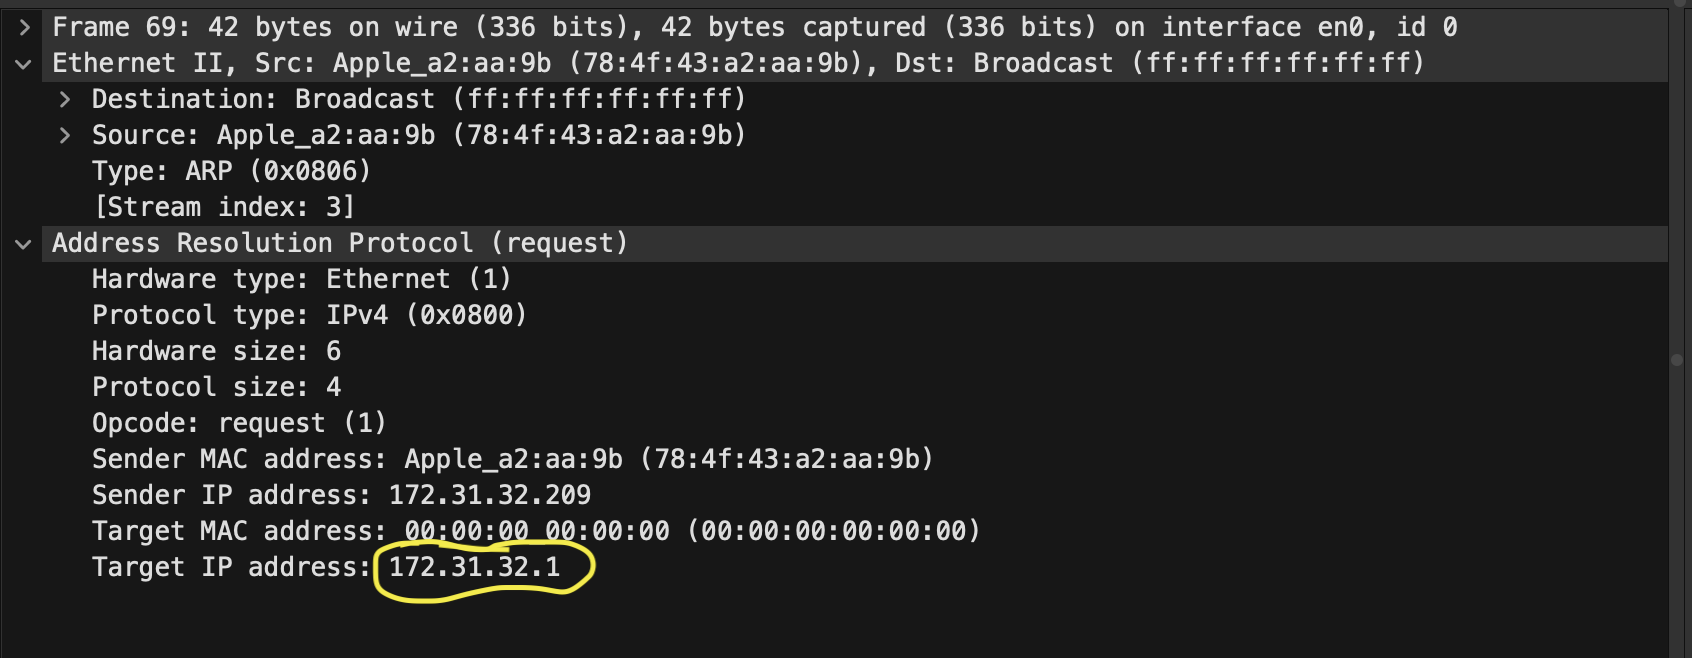
\includegraphics[scale=0.5]{Bilder/request_paket.png}
	\caption{ARP Request Paket. Die gesuchte IP Adresse in gelb}
	\end{figure}
	\begin{figure}[H]
	\centering
	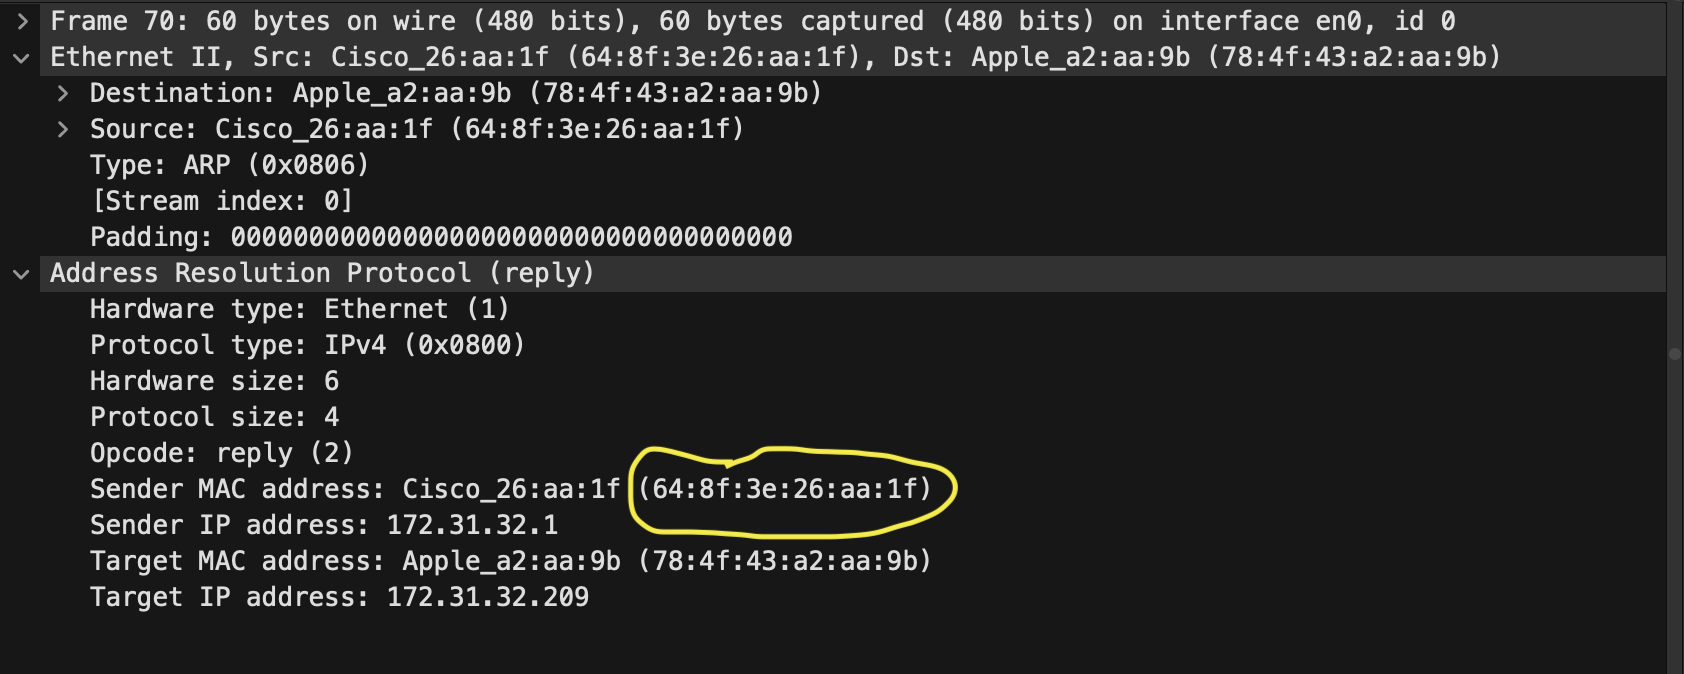
\includegraphics[scale=0.5]{Bilder/reply_paket.png}
	\caption{ARP Reply Paket. Sender MAC Adresse ebenfalls in gelb.}
	\end{figure}
	\section{Ping}
	\cprotect\subsection{Was ist \verb|ping|? }
	Ping sendet wiederholt ICMP Pakete an die Zieladresse und erbittet um Antwort. So kann man zum Beispiel herausfinden ob man selbst eine Verbindung hat oder ob ein anderer Teilnehmer im Netzwerk erreichbar ist.
	\subsection{Ping - Command Line}
	\begin{figure}[H]
	\centering
	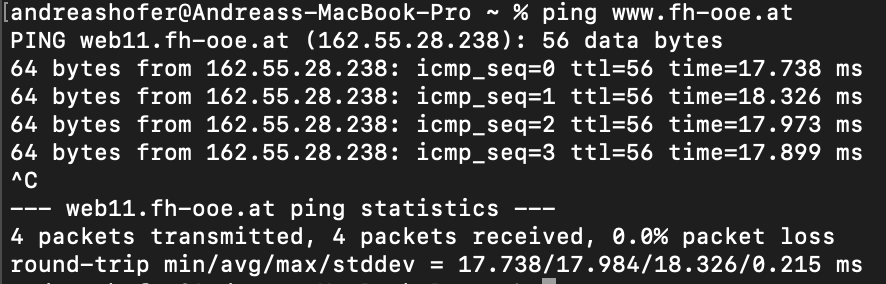
\includegraphics[scale=0.6]{Bilder/ping_terminal.png}
	\caption{Command Line des Pings an fh-ooe.at}
	\end{figure}
	\subsection{Ping - Wireshark request/reply Paar}
	\begin{figure}[H]
	\centering
	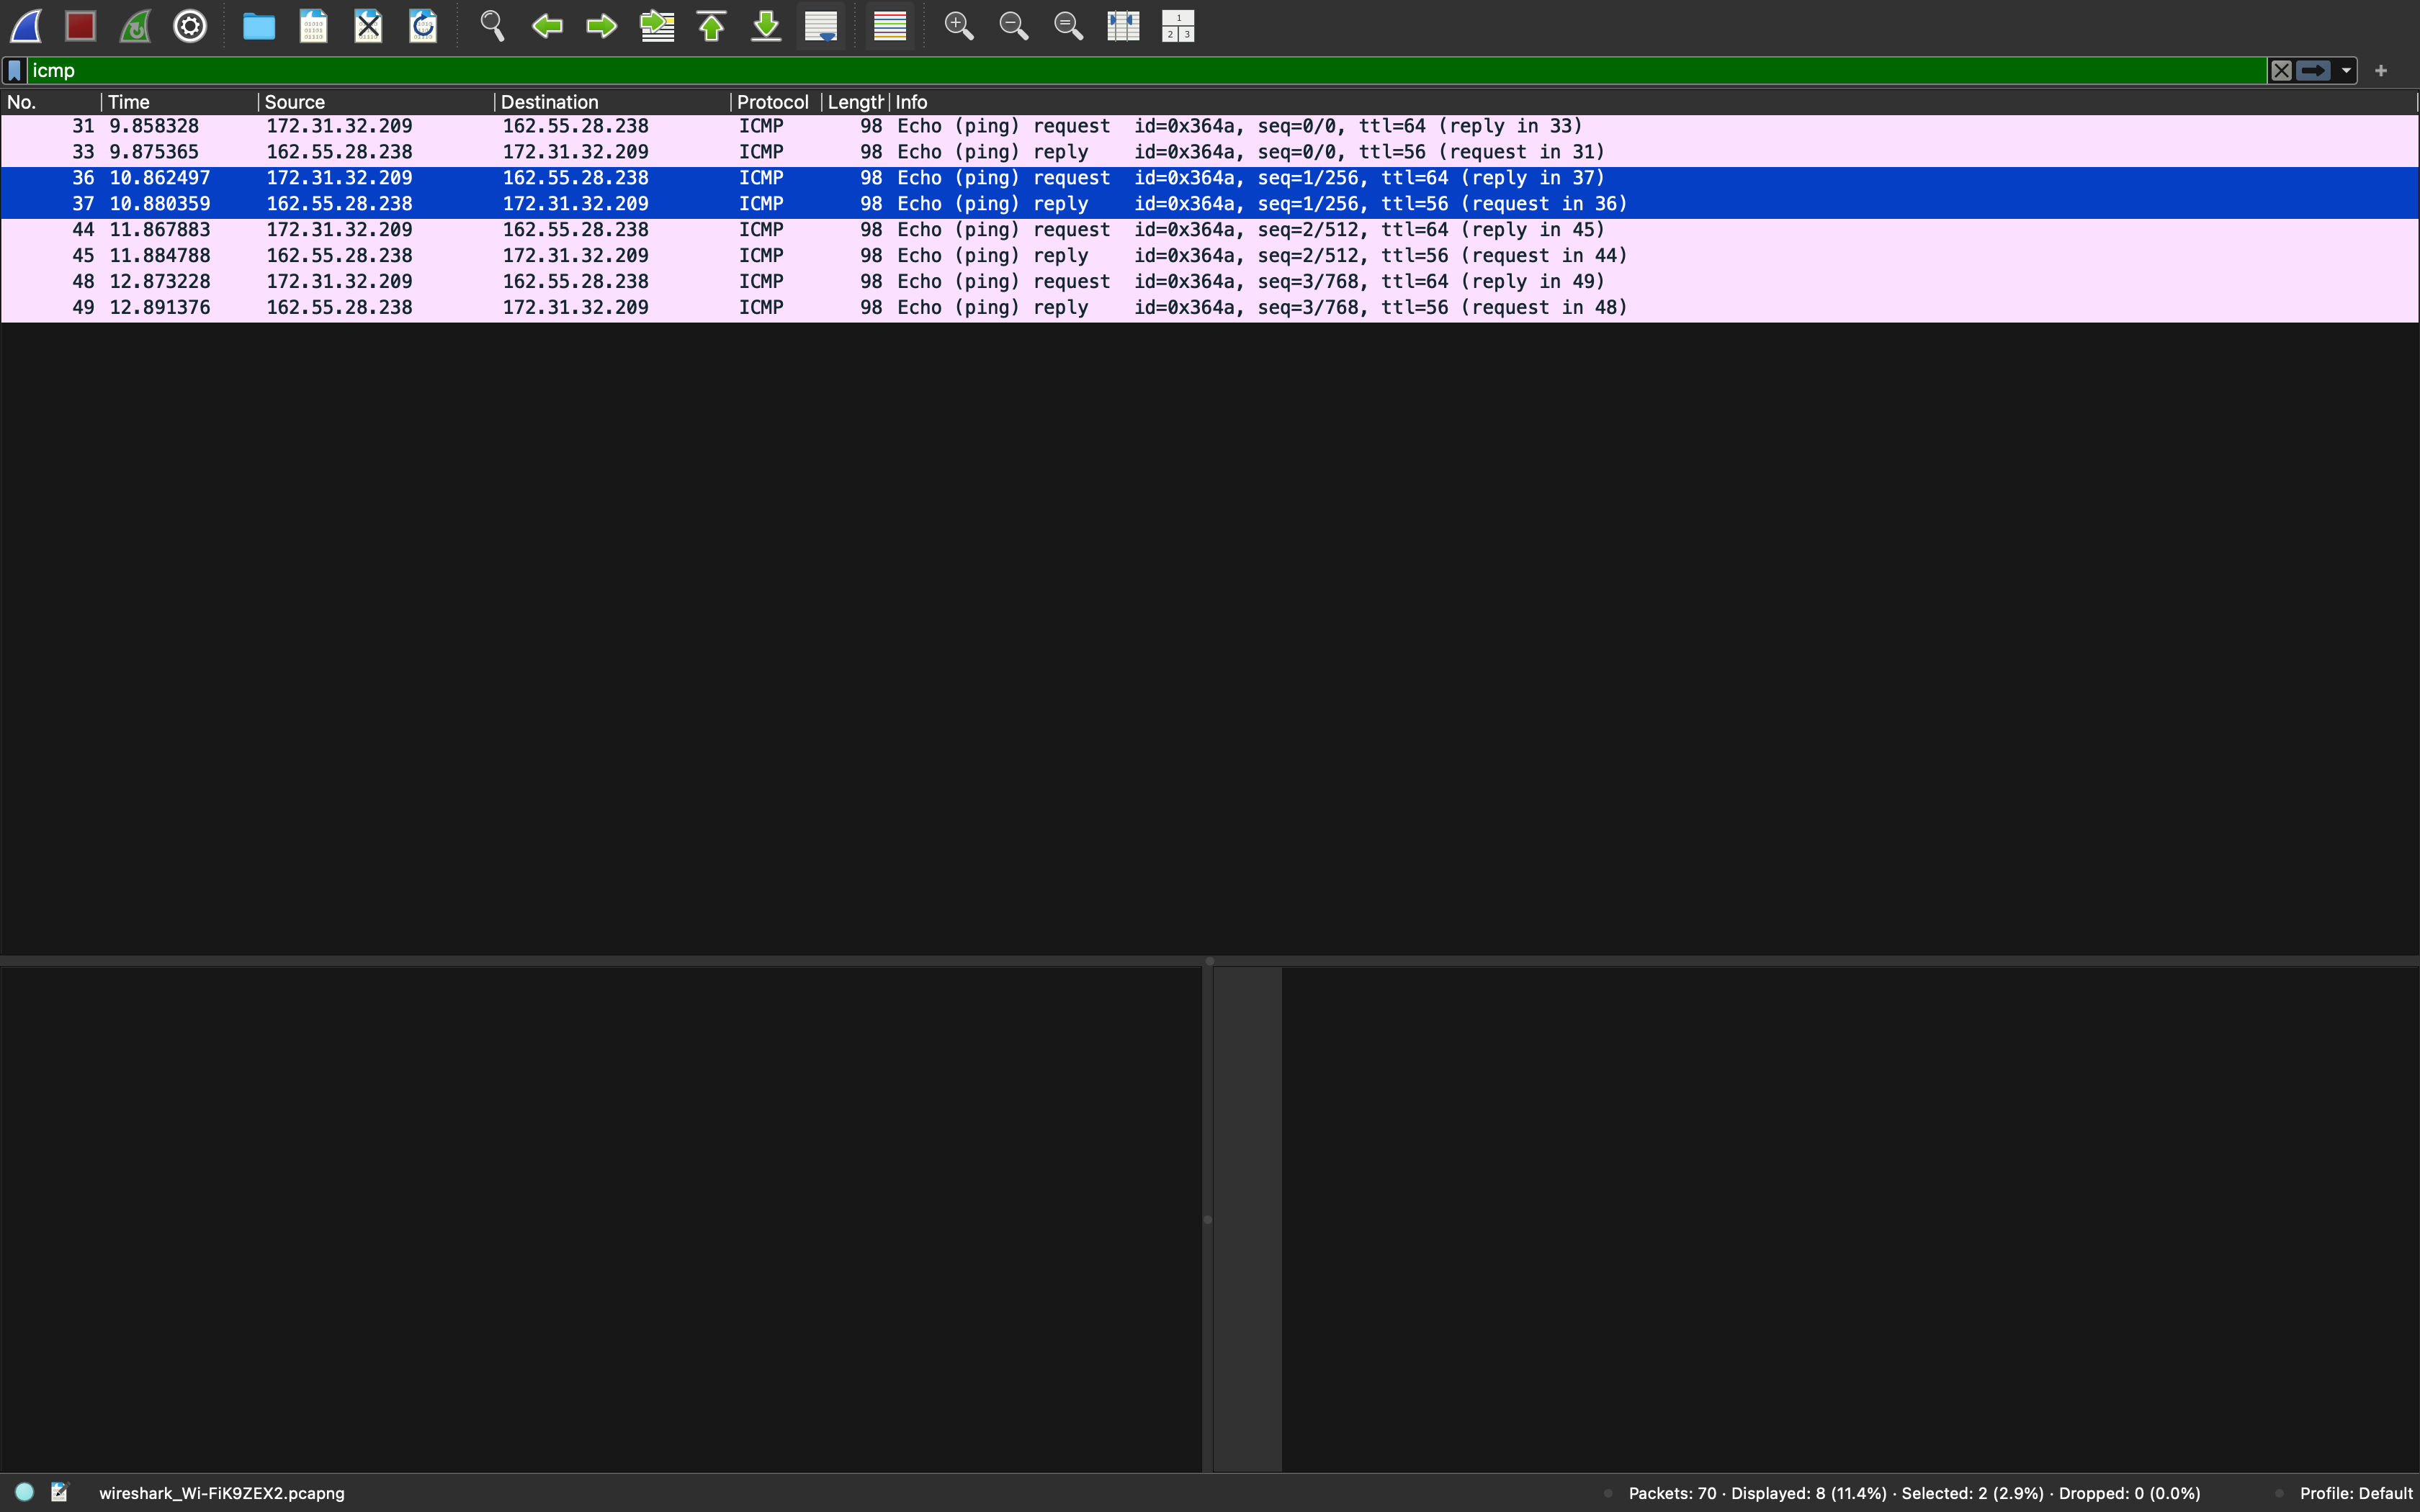
\includegraphics[scale=0.3]{Bilder/ping_request.png}
	\caption{Wireshark output des Pings. Markiert ein request/reply Paar.}
	\end{figure}
	\subsection{Ping - Time-To-Live}
	\begin{figure}[H]
	\centering
	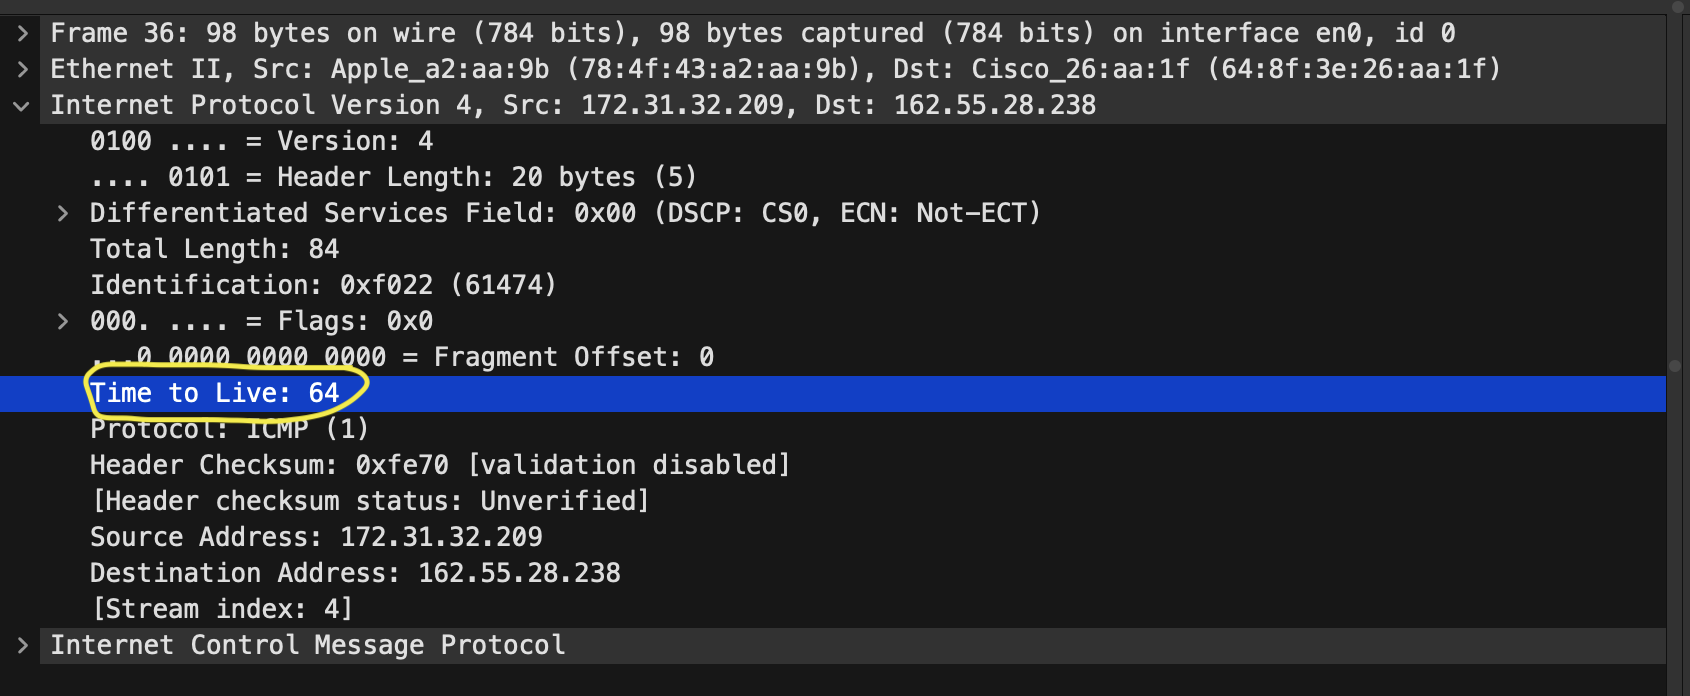
\includegraphics[scale=0.5]{Bilder/ping_paket.png}
	\caption{Ping request Paket. Time to Live in gelb.}
	\end{figure}
	\subsection{Was ist Time-To-Live?}
	Time to Live gibt an, wie oft ein Paket weitergeleitet wird, bevor ein Router es verwirft. Da jeder Router die TTL um 1 verringert und es nicht weiterleitet, falls dieser 0 erreicht hat, wird verhindert, dass Pakete ohne erreichbares Ziel ewig im Netzwerk existieren.
	\section{Ping unterschiedlicher IP-Adressen.}
	\begin{figure}[H]
	\centering
	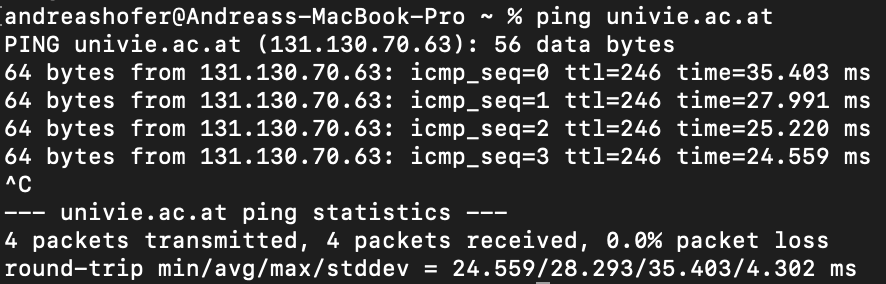
\includegraphics[scale=0.6]{Bilder/uniwien.png} \\
	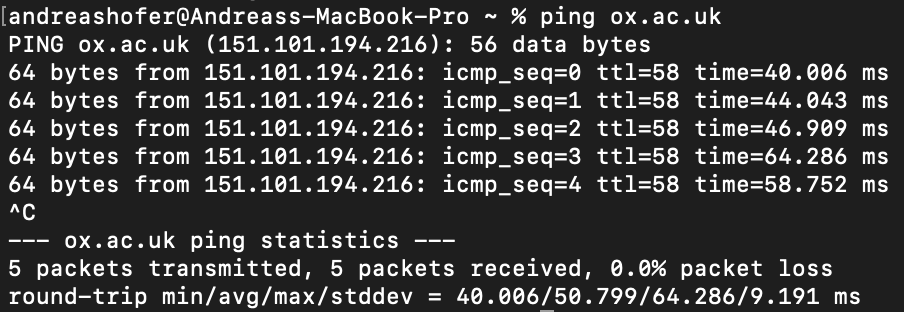
\includegraphics[scale=0.589]{Bilder/oxford.png} \\
	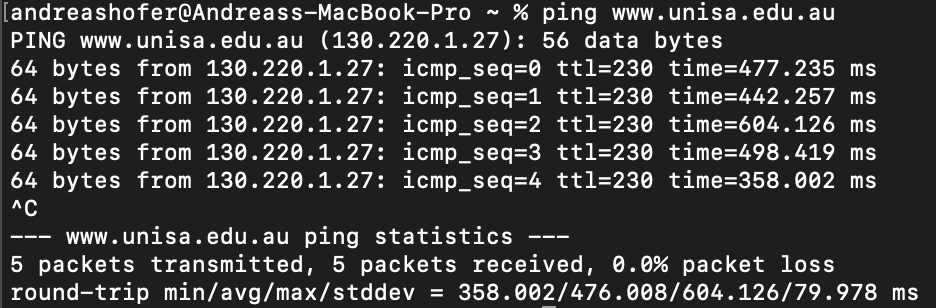
\includegraphics[scale=0.57]{Bilder/australien.png}\\
	\caption{Pings an die Uni Wien, Oxford und Australien}
	\end{figure}
	\paragraphlb{Zeiten zwischen Pings}
	Wieso die Round Trip Times bei dem gleichen Ziel immer unterschiedlich ist lässt sich eventuell dadurch erklären, dass jeder Router auf dem Weg zum Ziel eine kleine Latenz hinzufügt, falls er nicht sofort verfügbar ist. Andererseits könnte der Umstand, dass ein Paket bei jedem Ping eventuell eine andere Route zurücklegt auch zu unterschiedlichen Zeiten führen.
	\paragraphlb{Zeiten zwischen Universitäten}
	Dass die Universität in Australien im Allgemeinen eine höhere Round Trip Time hat, hängt höchstwahrscheinlich an der großen Distanz. Eventuell muss das Paket auch große Umwege machen, falls der direkteste Weg nicht verfügbar ist und so zum Beispiel versucht über Südamerika nach Australien zu gelangen.

	
	
	




















	
	
	
	
\end{document}